\documentclass[convert]{standalone}

\usepackage{tikz}
\usepackage{graphicx}
\pagestyle{empty}

% INT_AY20_MP1_L26_Fig03-Colliding_spheres.png

\begin{document}
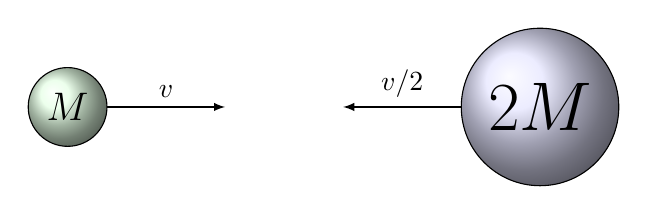
\begin{tikzpicture}[> = latex]

	% Colliding spheres
	
	\filldraw [ball color = green!10] (-3, 0) circle (0.5 cm) node [font = \Large] {$M$};
	\filldraw [ball color = blue!10] (3, 0) circle (1 cm) node [font = \Huge] {$2M$};
	
	% Velocity vectors
	
	\draw [->] (-2.5, 0) -- node [above] {$v$} (-1, 0);
	\draw [->] (2, 0) -- node [above] {$v/2$} (0.5, 0);
	
\end{tikzpicture}
\end{document}